\documentclass[class=minimal,border=0pt, 11pt]{standalone}
\usepackage{xcolor}
\usepackage{amsmath, amsfonts, mathtools, amssymb, amsthm} 
\usepackage{tikz, pgfplots}
\pgfplotsset{compat=1.8}
\DeclareMathOperator{\parab}{par}
\definecolor{darkgreen}{rgb}{0.0 0.5 0.0}
\definecolor{whitegreen}{rgb}{0.0 0.75 0.0}
\definecolor{whiteblue}{rgb}{0.0 0.0 1.2}
\definecolor{darkred}{rgb}{0.8 0.0 0.0}
\def\samplepar{10}
\def\sampleatn{30}
\def\samplesamp{35}


\makeatletter
\newcommand*{\circled}{\@ifstar\circledstar\circlednostar}
\newcommand*{\squared}{\@ifstar\squaredstar\squarednostar}
\makeatother

\newcommand*\circledstar[1]{%
  \tikz[baseline=(C.base)]
    \node[%
      fill,
      circle,
      minimum size=1.em,
      text=white,
%      font=\sffamily,
      inner sep=0.5pt
    ](C) {\texttt{#1}};%
}
\newcommand*\circlednostar[1]{%
  \tikz[baseline=(C.base)]
    \node[%
      draw,
      circle,
      minimum size=1.em,
%      font=\sffamily,
      inner sep=0.5pt
    ](C) {\texttt{#1}};%
}
\newcommand*\squaredstar[1]{%
  \tikz[baseline=(C.base)]
    \node[%
      fill,
      rectangle,
      minimum size=1.em,
      text=white,
%      font=\sffamily,
      inner sep=0.5pt
    ](C) {\texttt{#1}};%
}
\newcommand*\squarednostar[1]{%
  \tikz[baseline=(C.base)]
    \node[%
      draw,
      rectangle,
      minimum size=1.em,
%      font=\sffamily,
      inner sep=0.5pt
    ](C) {\texttt{#1}};%
}

\begin{document} 
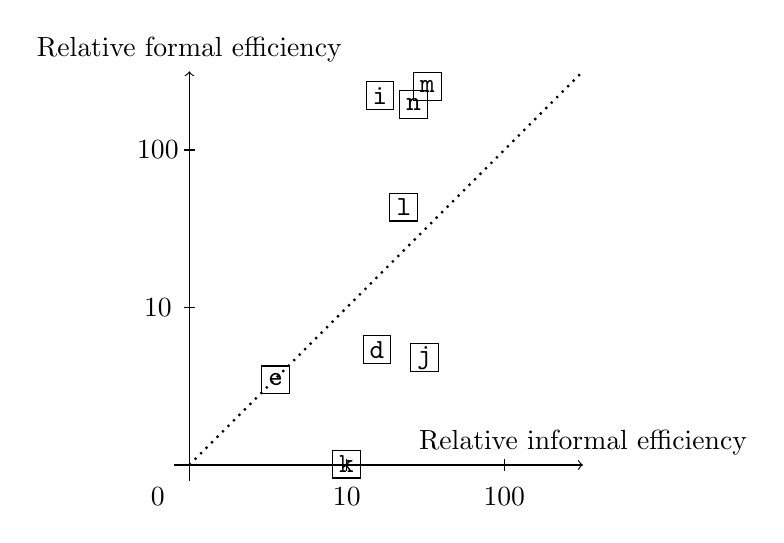
\begin{tikzpicture}[yscale=2, xscale=2]

\draw[->] (-0.1,0) -- (2.5,0) node[above] {Relative informal efficiency};
\draw[->] (0,-0.1) -- (0,2.5) node[above] {Relative formal efficiency};


\draw (1.191730, 0.732660) node {\squared{d}};

\draw (0.547977, 0.540454) node {\squared{e}};

\draw (1.210494, 2.345441) node {\squared{i}};

\draw (1.492916, 0.680888) node {\squared{j}};

\draw (0.997985, 0.005418) node {\squared{k}};

\draw (1.361728, 1.637213) node {\squared{l}};

\draw (1.511047, 2.402279) node {\squared{m}};

\draw (1.424538, 2.287272) node {\squared{n}};


\draw[domain=0:2.5, samples=80, dotted, thick] plot (\x,{\x}) node[anchor = south east] {$ $};
\draw (-0.2,-0.2) node {$0$}; 
\draw (1,1pt) -- (1,-1pt); \draw (1,-0.2) node {$10$}; 
\draw (2,1pt) -- (2,-1pt); \draw (2,-0.2) node {$100$}; 

\draw (1pt,1) -- (-1pt, 1); \draw (-0.2,1) node {$10$}; 
\draw (1pt,2) -- (-1pt, 2); \draw (-0.2,2) node {$100$}; 

\end{tikzpicture}
 \end{document}

\if{
let slog x = log (x) /. log(10.);;
let trel treal2float tfptaylor treal2floatformal tfptaylorformal = ( tfptaylor /.treal2float ), ( tfptaylorformal /.treal2floatformal) ;;

let terel i treal2float tfptaylor treal2floatformal tfptaylorformal  = 
let a, b = trel treal2float tfptaylor treal2floatformal tfptaylorformal in 
Printf.sprintf "
\\draw (%f, %f) node {\\squared{%c}};
" 
(slog(a)) (slog(b)) i ;;

let s4 = terel 'd' 0.40  6.22 3.016666 16.3  in
let s5 = terel 'e'  2.37  8.37 15.376 53.37  in
let s9 = terel 'i'  0.93  15.1 0.333  73.771 in
let s10 = terel 'j'  3.15  98.0 31.73 152.18  in
let s11 = terel 'k'  21.6  215.0 454.42   460.125 in
let s12 = terel 'l'  0.42   9.66 1.63  70.697  in
let s13 = terel 'm'  0.16  5.19 0.0733 18.509   in
let s14 = terel 'n'  0.38   10.1 0.1666 32.281 in
print_endline (s4^s5^s9 ^ s10 ^ s11 ^ s12 ^ s13 ^s14);;

}\fi
